% Created 2018-03-14 Wed 15:32
% Intended LaTeX compiler: pdflatex
\documentclass[presentation]{beamer}
\usepackage[utf8]{inputenc}
\usepackage[T1]{fontenc}
\usepackage{graphicx}
\usepackage{grffile}
\usepackage{longtable}
\usepackage{wrapfig}
\usepackage{rotating}
\usepackage[normalem]{ulem}
\usepackage{amsmath}
\usepackage{textcomp}
\usepackage{amssymb}
\usepackage{capt-of}
\usepackage[colorlinks=true]{hyperref}
\usetheme{default}
\usecolortheme{}
\usefonttheme{}
\useinnertheme{}
\useoutertheme{}
\author{Paul Feitzinger}
\date{\today}
\title{Redefine Success, Redefine Relevance.}

\hypersetup{
 pdfauthor={Paul Feitzinger},
 pdftitle={Redefine Success, Redefine Relevance.},
 pdfkeywords={},
 pdfsubject={},
 pdfcreator={Emacs 25.3.1 (Org mode 9.0.1)},
 pdflang={English}}
\begin{document}

\maketitle

\begin{frame}[label={sec:org543d9ec}]{So much irrelevance}
\begin{figure}[htbp]
\centering
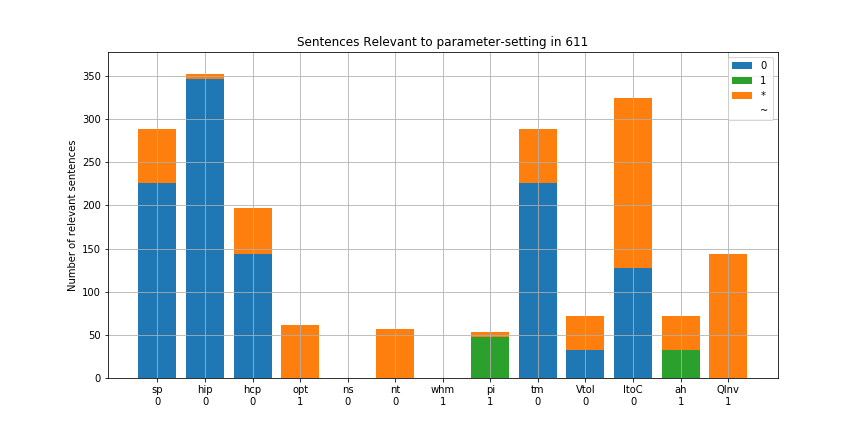
\includegraphics[width=.9\linewidth]{./images/english-triggers.png}
\end{figure}
\begin{itemize}
\item Read the left-most bar of this graph like this: "Out of the 360 colag
english sentences, there were 225 global triggers for SP=0, and 100ish
sentences that were ambiguously relevant to its value-setting. The rest were
irrelevant."
\item Notably, "There are no languages in Colag English relevant to Null Subject
or Wh-movement."
\end{itemize}
\end{frame}
\begin{frame}[label={sec:org27051ad}]{But look, the NDL can see NS and WHM!}
\begin{center}
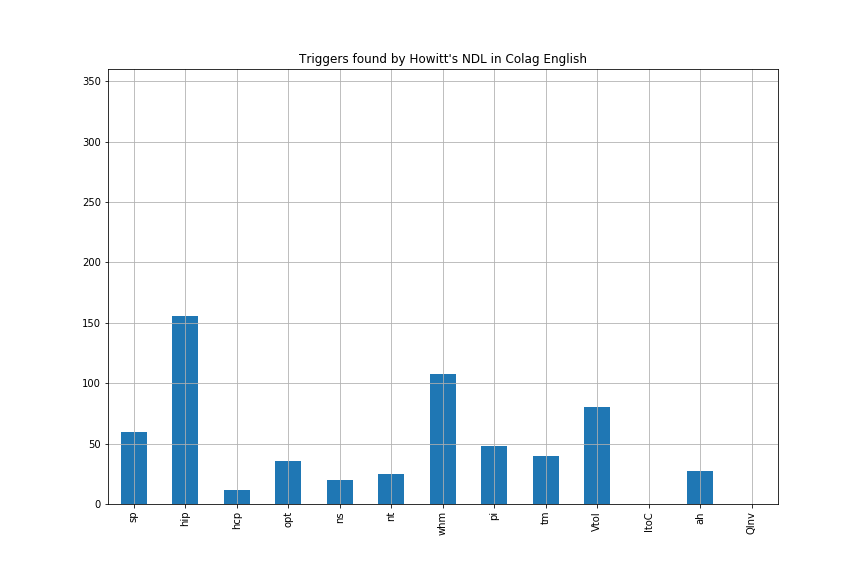
\includegraphics[width=.9\linewidth]{./images/ndl-triggers.png}
\end{center}
\end{frame}
\begin{frame}[shrink=12,label={sec:orgc63b381}]{Our definition of irrelevant}
\begin{itemize}
\item Our algorithm considers a sentence \(s\) irrelevant to a parameter \(p\) when it
fails to find a single example of where toggling \(p\) in any of the grammars
that license \(s\), causes \(s\) to no longer be licensed.
\end{itemize}

\begin{align*}
G_{sent} &= \text{the set of grammars that license sentence $sent$} \\
g_p &= \text{The value of param $p$ in grammar $g$} \\
pair_p^g &= \text{The minimal pair of $g$ on param $p$ (aka $g$ with $p$ toggled)} \\
  Trig(sent) &= \begin{bmatrix} Trig(sent, p) : p \in 1..13 \end{bmatrix} \\
  Trig(sent, p) &= \left\{\begin{array}{lr}
      0                        & \iff \{g_p : g \in G_{sent} \} = \{0\} \\
      1                        & \iff \{g_p : g \in G_{sent} \} = \{1\}\\
      Irrel?(G_{sent}, p) & \iff \{g_p : g \in G_{sent} \} = \{0, 1\} \\
      \end{array}\right\} \\
Irrel?(G_{sent}, p) &= \left\{\begin{array}{lr}
      Ambig                        & \iff \exists g \in G_{sent} :
                                     (pair_p^g \notin G_{sent}) \cap (pair_p^g \in G) \\
      Irrel                        & \iff  otherwise \\
      \end{array}\right\} \\
\end{align*}
\end{frame}
\begin{frame}[label={sec:orgb2ce0ff}]{Weakly equivalent, hamming distance of 1}
\begin{itemize}
\item But this means any language \(L\) with a weakly equivalent language \(L'\),
where then hamming distance between \(L\) and \(L'\) = 1, will cause lots of
irrelevance in sentences. \begin{center}
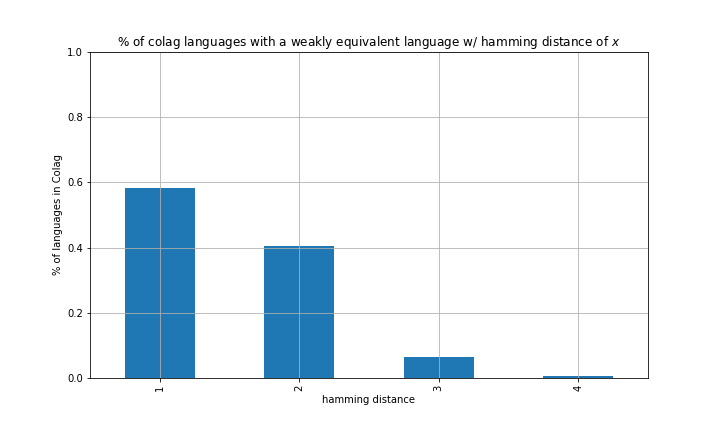
\includegraphics[width=.9\linewidth]{./images/weak-equiv-ham-dist.png}
\end{center}
\item which describes 60\% of the languages in Colag.
\end{itemize}
\end{frame}
\begin{frame}[label={sec:orgcabe6ad}]{Learning \(g\) exactly}
\begin{center}
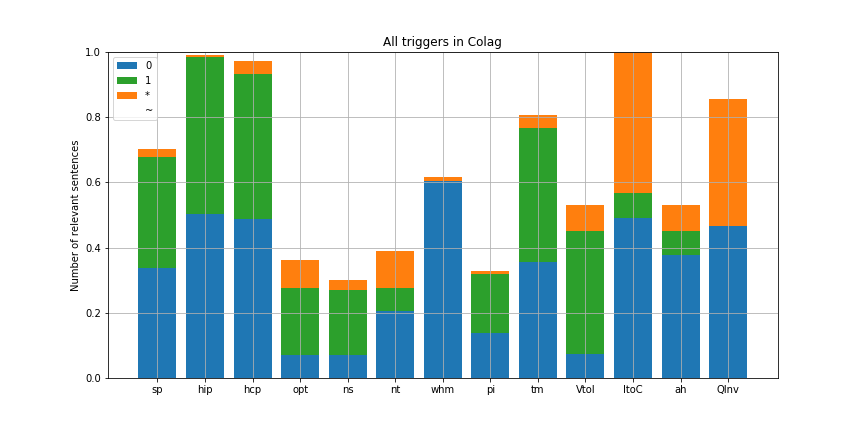
\includegraphics[width=.9\linewidth]{./images/all-triggers.png}
\end{center}
\begin{itemize}
\item What we're really saying is, if we define successful learning to mean
"seeing a sample of \(L(g)\) and arriving at \(g\) exactly", then these are how
many strong, ambiguous, and irrelevant triggers exist for arriving at that
hypothesis.
\end{itemize}
\end{frame}
\begin{frame}[label={sec:org6662404}]{Learning \(g\) exactly}
\begin{itemize}
\item But that requires our learner to be able to differentiate between weakly
equivalent languages \footnote{languages where \(L(g) = L(g')\) - the set of
sentences generated by \(g\) and \(g'\) are exactly the same (though not
necessarily the parses of those sentences).}
\item We don't claim our learners can actually do this (besides the TLA?), so
perhaps we should relax our definition of successful learning when computing
the per-parameter triggers.
\end{itemize}
\end{frame}
\begin{frame}[shrink=12,label={sec:org09bd30d}]{Learning \(g\) or a Weak Equivalent}
\begin{itemize}
\item This algorithm finds \(s\) irrelevant to \(p\) when it fails to find a single
example of when toggling \(p\) in any of the \emph{non-g-equivalent-grammars} that
license \(s\), causes \(s\) to no longer be licensed.
\end{itemize}
\begin{align*}
G_{sent} &= \text{the set of grammars that license sentence $sent$} \\
W_g &= \text{the set of grammars weakly equivalent to $g$} \\
\bar{W}_{sent}^g &= \text{the grammars that license $sent$, excluding $W_g$} \\
g_p &= \text{The value of param $p$ in grammar $g$} \\
pair_p^g &= \text{The minimal pair of $g$ on param $p$ (aka $g$ with $p$ toggled)} \\
  Trig(sent) &= \begin{bmatrix} Trig(sent, p) : p \in 1..13 \end{bmatrix} \\
  Trig(sent, p) &= \left\{\begin{array}{lr}
      0                        & \iff \{g_p : g \in G_{sent} \} = \{0\} \\
      1                        & \iff \{g_p : g \in G_{sent} \} = \{1\}\\
      Irrel?(G_{sent}, p) & \iff \{g_p : g \in G_{sent} \} = \{0, 1\} \\
      \end{array}\right\} \\
Irrel?(G_{sent}, p) &= \left\{\begin{array}{lr}
      Ambig                        & \iff \exists g \in G_{sent} :
                                     (pair_p^g \notin \bar{W}_{sent}^g) \cap (pair_p^g \in G) \\
      Irrel                        & \iff  otherwise \\
      \end{array}\right\} \\
\end{align*}
\end{frame}
\begin{frame}[label={sec:orgdb06441}]{Learning \(g\) or a Weak Equivalent}
\begin{center}
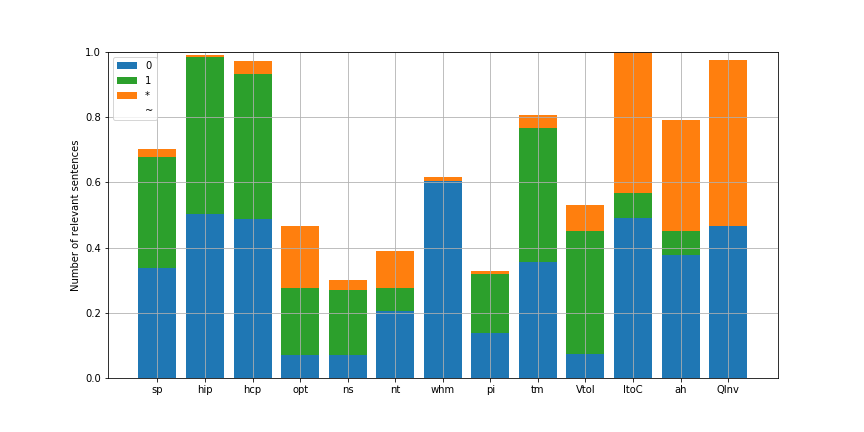
\includegraphics[width=.9\linewidth]{./images/all-triggers-weak-equiv.png}
\end{center}

\begin{itemize}
\item If we settle for learning either \(G\) or a weakly equivalent language, then
the following number of sentences go from irrelevant to ambiguously
relevant.
\begin{center}
\begin{tabular}{rrlr}
opt & ItoC & ah & QInv\\
\hline
5047 & 71 & 12,591 & 5732\\
\end{tabular}
\end{center}
\end{itemize}
\end{frame}
\begin{frame}[label={sec:orgff0c87a}]{Learning \(g\) or a Weak Equivalent}
\begin{itemize}
\item Here's how Colag English looks under that definition:
\end{itemize}

\begin{center}
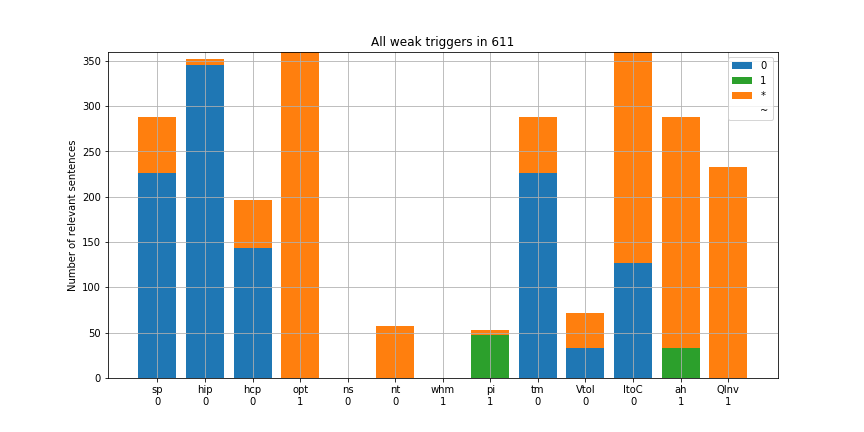
\includegraphics[width=.9\linewidth]{./images/english-triggers-weak-equiv.png}
\end{center}
\end{frame}

\begin{frame}[label={sec:org87caaf5}]{Superset relation, hamming distance of 1}
\begin{itemize}
\item It's also the case that any \(g\) with a hamming-distance-1 superset language
will cause irrelevance to be assigned to many sentences:

\begin{center}
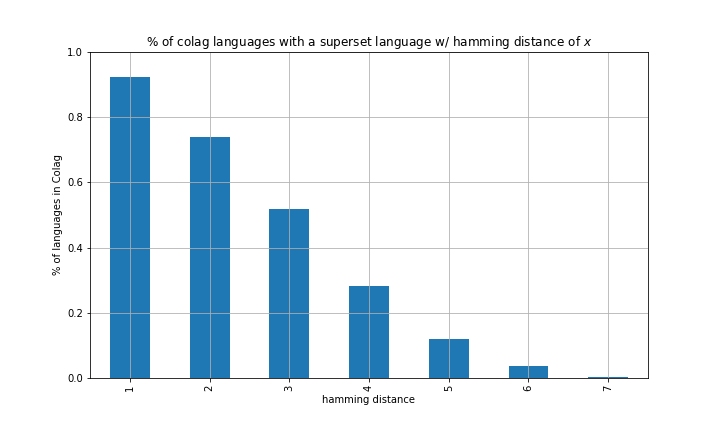
\includegraphics[width=.9\linewidth]{./images/superset-ham-dist.png}
\end{center}
\end{itemize}
\end{frame}
\begin{frame}[shrink=12,label={sec:org2530460}]{Learning \(g\) or any Superset}
\begin{itemize}
\item We could lower the bar even further and say that we've succeeded if we learn
\(g\) or any of its subset languages.
\item This algorithm finds \(s\) irrelevant to \(p\) when it fails to find a single
example of when toggling \(p\) in any of the \emph{non-g-subset-grammars} that
license \(s\), causes \(s\) to no longer be licensed.
\end{itemize}

\begin{align*}
G_{sent} &= \text{the set of grammars that license sentence $sent$} \\
S_g &= \text{the set of grammars in superset relation to $g$} \\
\bar{S}_{sent}^g &= \text{the grammars that license $sent$, excluding $S_g$} \\
g_p &= \text{The value of param $p$ in grammar $g$} \\
pair_p^g &= \text{The minimal pair of $g$ on param $p$ (aka $g$ with $p$ toggled)} \\
  Trig(sent) &= \begin{bmatrix} Trig(sent, p) : p \in 1..13 \end{bmatrix} \\
  Trig(sent, p) &= \left\{\begin{array}{lr}
      0                        & \iff \{g_p : g \in G_{sent} \} = \{0\} \\
      1                        & \iff \{g_p : g \in G_{sent} \} = \{1\}\\
      Irrel?(G_{sent}, p) & \iff \{g_p : g \in G_{sent} \} = \{0, 1\} \\
      \end{array}\right\} \\
Irrel?(G_{sent}, p) &= \left\{\begin{array}{lr}
      Ambig                        & \iff \exists g \in G_{sent} :
                                     (pair_p^g \notin \bar{S}_{sent}^g) \cap (pair_p^g \in G) \\
      Irrel                        & \iff  otherwise \\
      \end{array}\right\} \\
\end{align*}
\end{frame}
\begin{frame}[label={sec:org4192c68}]{Learning \(g\) or any Superset}
\begin{center}
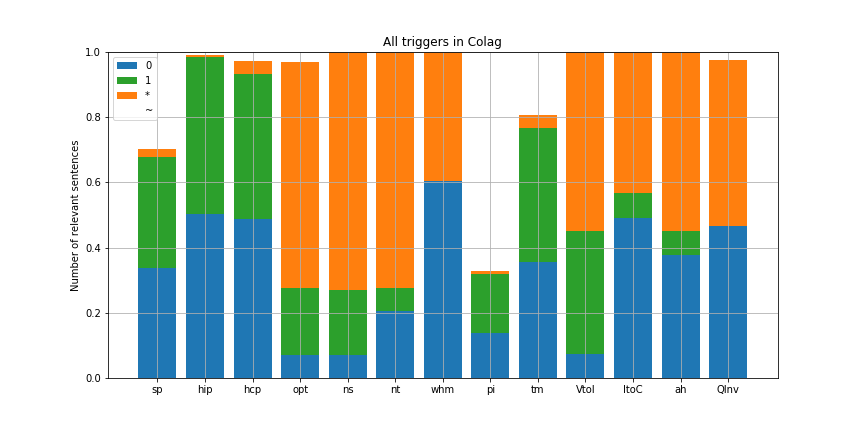
\includegraphics[width=.9\linewidth]{./images/all-triggers-supersets.png}
\end{center}

\begin{itemize}
\item Here's how many relevant sentences we "gain" by doing that:
\end{itemize}

\begin{center}
\begin{tabular}{lllllrll}
opt & ns & nt & whm & VtoI & ItoC & ah & QInv\\
29,195 & 33,629 & 29,429 & 18,421 & 22,647 & 71 & 22,647 & 5,732\\
\end{tabular}
\end{center}
\end{frame}
\begin{frame}[label={sec:org2ade7b4}]{Learning \(g\) or any Superset}
\begin{itemize}
\item Here's how Colag English looks under that definition:
\end{itemize}

\begin{center}
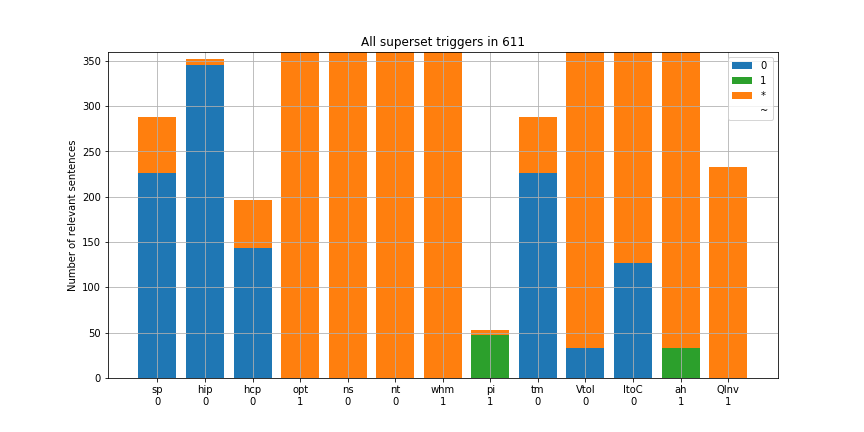
\includegraphics[width=.9\linewidth]{./images/english-triggers-supersets.png}
\end{center}
\end{frame}
\end{document}
